\documentclass[course=asp]{aspdoc}
\usepackage{graphicx}
\graphicspath{{./Bilder/}}

\newcommand{\theGroup}{team 117} % Beispiel: 42
\newcommand{\theNumber}{502: XTEA}
\author{Guo, Linfeng\\Gönenc, Hazar \\Özakay, Baris}
\date{Wintersemester 2021/22}


% Diese Zeile bitte -nicht- aendern.
\title{Gruppe \theGroup{} -- Abgabe zu Aufgabe \theNumber}

\begin{document}
\maketitle



\section{Einleitung}
Im Rahmen unseres Projektes im Fach Aspekte der systemnahen Programmierung bei der Spieleentwicklung war es unsere Aufgabe einen Ver- und Entschlüsselungsalgorithmus XTEA in Assemblercode und C zu implementieren, die Korrektheit der Implementierung zu überprüfen und die Performanz von unterschiedlichen XTEA-Implementierungen zu vergleichen und zu analysieren. Diese Aufgabe lässt sich in folgende Bereiche aufteilen: Konzeption, die Funktionsweise des XTEA Algorithmus, Verfahren für die Optimierung des Algorithmus verstehen und den XTEA Algorithmus in Assemblercode zu implementieren. Die Bearbeitung dieser Teilbereiche wird im Folgenden beschrieben.  \\

\newpage
\section{Lösungsansatz}
\subsection*{2.1.Feistelchiffre }
Der XTEA Algorithmus ist ein Ver -und Entschlüsselungsalgorithmus, welcher auf der Struktur von Feistelchiffre basiert. Feistelchiffre ist eine Struktur, die für die symmetrische Verschlüsselung verwendet wird. Unter symmetrischer Verschlüsselung ist zu verstehen, dass für die Ver- und Entschlüsselung nur ein Schlüssel verwendet wird. Wir würden daher erstmal mit Feistelchiffre, der Grundstruktur der symmetrischen Verschlüsselung, eingehen.\\
Feistelchiffre lässt sich in vier Schritte aufteilen. Zuerst hat man ein Klartextblock mit der Datei, welche meist acht Bytes ist und teilt diese in zwei gleich große Bl\"ocke L0 und R0, die vier Bytes entsprechen auf.

\begin{table}[H]
\centering
    \begin{tabular}{|l|l|l|l|l|l|l|l|}
        \hline
        B & E & I & S & P & I & E & L   \\
        \hline
    \end{tabular}
    \caption{Nachricht}
\end{table}

\begin{table}[H]
\centering
    \begin{tabular}{|l|l|l|l|l|l|l|l|}
        \hline
        42 & 45 & 49 & 53 & 50 & 49 & 45 & 4C   \\
        \hline
    \end{tabular}
    \caption{Nachricht in Hex Code}
\end{table}



\begin{table}[H]

    \begin{minipage}{.5\linewidth}

      \centering
        \begin{tabular}{|l|l|l|l|}
		\hline
            42 & 45 & 49 & 53   \\
		\hline
        \end{tabular}

	\caption{L0}
    \end{minipage}%
    \begin{minipage}{.5\linewidth}

 \centering

        \begin{tabular}{|l|l|l|l|}
           \hline
		 50 & 49 & 45 & 4C   \\
		\hline
        \end{tabular}
\caption{R0}
    \end{minipage}
\end{table}
Danach findet die eigentliche Verschlüsselung statt. Man führt die Verschlüsselungsfunktion mit dem Schlüssel, der ebenfalls vier Bytes entspricht, auf R0 aus. Die Funktion bei Feistelchiffre ist allerdings undefiniert da Feistelchiffre nur die Struktur anbietet. Der Wert der sich durch die Funktion ergibt, wird anschließend mit dem linken Teil durch die XOR- Operation eingefangen. So ergibt sich das neue R1. Die ursprüngliche R0 wird dann zu L1. Nach jeder Verschlüsselung wird die Position vom linken und dem rechten Block getauscht, wie oben beschrieben wird.\\
Die Entschlüsselung funktioniert im Prinzip genau wie die Verschlüsselung. Nur mit dem Unterschied, dass man die Position vom linken und rechten Teil tauscht. Also wird Ln+1 in die Funktion mit dem gleichen Key eingesetzt. Das Ergebnis wird dann mit Rn+1 per XOR abgebildet. Der Wert wird dann zu Rn und Ln+1 wird zu Ln.~\cite{feistelchipher}

\begin{figure}[h]
\centering
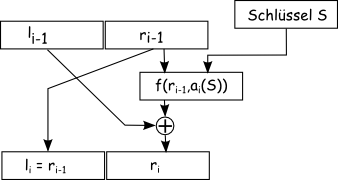
\includegraphics[scale = 0.4]{feistel.png}
\caption{Feistelchiffre}
\end{figure}
\newpage


\subsection*{2.2.XTEA}
Die Aufgabe des Projekts liegt darin, den XTEA Algorithmus sowohl in C als auch in Assembler zu implementieren. Für die Implementierung des XTEA Algorithmus sollte man zunächst wissen wie XTEA überhaupt funktioniert. \\
Das Verfahren von XTea ist eine weiteire Entwicklung von TEA und ist auf Feistelchiffre basiert. Der eingelesene Wert, welcher acht Bytes entspricht, wird in zwei Blöcke aufgeteilt: V1 und V2. Der Schlüssel bei XTEA beträgt 16 Bytes und wird in vier Teile aufgeteilt, die jeweils vier Bytes entsprechen. Für XTEA brauchen wir zusätzlich noch eine weitere Variable s, die Summe die immer nach der Verschlüsselung von V1 mit der magischen Zahl ${\delta}$ addiert wird. ${\delta}$ lässt sich aus der Formel:
\begin{equation}
     \delta  =   \lfloor ( \surd 5 -1)  \cdot  2^{31} \rfloor
\end{equation}
berechnen. Jede Runde findet eine doppelte Verschlüsselung statt.~\cite{appel2016sicherheitsaspekte} \\
Man beginnt mit der Verschlüsselung von V1. Hier wird V2 in zwei Blöcken geshiftet, bitweiser Shift. Block 1: V2 << 4 und Block: V2 >>5. Die zwei Blöcke werden per XOR  zu einem Wert zusammengefügt, und mit V2 addiert. Danach wird das Ergebnis mit der Summe von s, welche am Anfang Null entspricht, und dem Schlüssel, dessen Index sich aus der Variable s Modulo drei ergibt per XOR abgebildet. Zum Schluss wird das Ergebnis auf V1 addiert. \\
Als Veranschaulichung nehmen wir wieder das Beispielwort "BEISPIEL", in Hex Code. Und teilen dieses Wort in V1 und V2 auf.
\begin{table}[H]

    \begin{minipage}{.5\linewidth}

      \centering
        \begin{tabular}{|l|l|l|l|}
		\hline
            42 & 45 & 49 & 53   \\
		\hline
        \end{tabular}

	\caption{V1}
    \end{minipage}%
    \begin{minipage}{.5\linewidth}

 \centering

        \begin{tabular}{|l|l|l|l|}
           \hline
		 50 & 49 & 45 & 4C   \\
		\hline
        \end{tabular}
\caption{V2}
    \end{minipage}
\end{table}

\begin{table}[H]
\centering
    \begin{tabular}{|l|l|l|l||l|l|l|l||l|l|l|l||l|l|l|l|}
        \hline
        41 & 53 & 50 & 41 & 53 & 50 & 41 & 53  & 50 & 41 & 53 & 50 & 41 & 53 & 50 & 41 \\
        \hline
    \end{tabular}
    \caption{Key}
\end{table}


Anschließend folgt das Shiften von V2 und die XOR Operation wird danach an den beiden Blöcken ausgeführt.
\begin{table}[H]

    \begin{minipage}{.5\linewidth}

      \centering
        \begin{tabular}{|l|l|l|l|}
		\hline
            04 & 94 & 54 & C0   \\
		\hline
        \end{tabular}

	\caption{V2 << 4}
    \end{minipage}%
    \begin{minipage}{.5\linewidth}

 \centering

        \begin{tabular}{|l|l|l|l|}
           \hline
		 02 & 82 & 4A & 2A   \\
		\hline
        \end{tabular}
\caption{V2 >> 5}
    \end{minipage}
\end{table}

\begin{table}[H]
\centering
    \begin{tabular}{|l|l|l|l|}
        \hline
        06 & 16 & 1E & EA    \\
        \hline
    \end{tabular}
    \caption{(V2 << 4) $\oplus$ (V2 >> 5)}
\end{table}
Das Ergebnis wird mit V2 addiert. Als nächstes wird die XOR Operation, zwischen dem Ergebnis und der Summe von s und Key, ausgeführt. Da bei der ersten Runde s immer Null ist wird K[0] genommen.
\begin{table}[H]
\centering
    \begin{tabular}{|l|l|l|l|}
        \hline
        56 & 5F & 64 & 36    \\
        \hline
    \end{tabular}
    \caption{((V2 << 4) $\oplus$ (V2 >> 5)) + V2}
\end{table}

\begin{table}[H]
\centering
    \begin{tabular}{|l|l|l|l|}
        \hline
        41 & 53 & 50 & 41    \\
        \hline
    \end{tabular}
    \caption{K[0]}
\end{table}

\begin{table}[H]
\centering
    \begin{tabular}{|l|l|l|l|}
        \hline
        17 & 0C & 34 & 77    \\
        \hline
    \end{tabular}
    \caption{(((V2 << 4) $\oplus$ (V2 >> 5)) + V2) $\oplus$ (s + K[s\& 3])}
\end{table}
Zum Schluss wird das Ergebnis zu V1 addiert.

\begin{table}[H]
\centering
    \begin{tabular}{|l|l|l|l|}
        \hline
        59 & 51 & 7D & CA    \\
        \hline
    \end{tabular}
    \caption{((((V2 << 4) $\oplus$ (V2 >> 5)) + V2) $\oplus$ (s + K[s\& 3])) + V1}
\end{table}



Die Variable s wird jetzt um die magische Zahl erhöht. Bei V2 funktioniert die Verschlüsselung ähnlich wie für V1. Wir teilen V1 durch das Shiften in zwei Blöcke auf, exakt wie bei der Verschlüsselung von V1 werden die zwei Blöcken per XOR zu einem neuen Ergebnis zusammengefügt und mit V1 addiert. Das Ergebnis verschlüsselt sich dann per XOR mit der Summe von s und der Schlüssel, dessen Index jetzt aus s shift 11 Modulo 3 besteht. Am Ende wird das Ergebnis auf V1 addiert.
\begin{figure}[h]
\centering
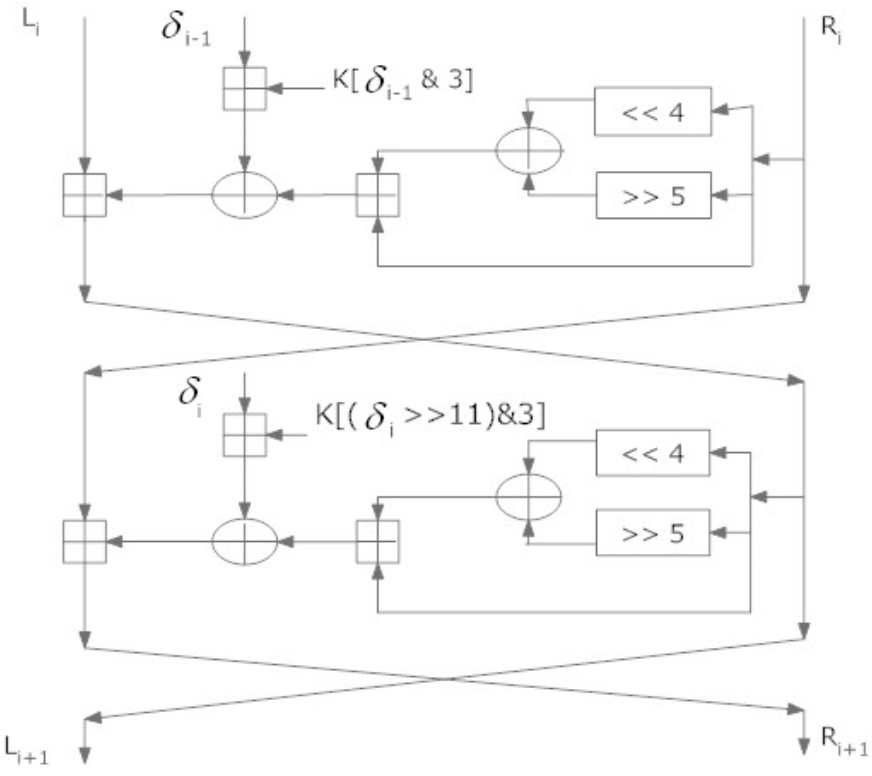
\includegraphics[scale = 0.55]{XTEA.png}
\caption{XTEA(${\delta}$ ist in dem Fall unser s)}
\end{figure}
\newpage




\newpage
\subsection*{2.3.Unterschiede und Gemeinsamkeiten zwischen XTEA und Feistelchiffre}
Die Vorgehensweise beider Verfahren haben Gemeinsamkeiten und Unterschiede. Da XTEA auf Feistelchiffre basiert verwendet man hier auch das symmetrische Verschlüsselungsverfahren, d.h. für die Ver- und Entschlüsselung der Nachricht wird derselben Schlüssel verwendet. Bei beiden werden am Anfang der Verschlüsselung die zu verschlüsselnden Daten in zwei Blöcke aufgeteilt und der Verschlüsselungsprozess kann mehrere Runden dauern. Die Länge der zu verschlüsselnden Daten muss immer ein Vielfaches der Blocklänge sein. Auch das Verwenden von XOR kann bei beiden Verfahren gefunden werden. \\
Es gibt aber auch Unterschiede zwischen beiden Verfahren. Bei XTEA findet jede Runde eine doppelte Verschlüsselung statt, was bei Feistelchiffre nicht zu finden ist. Außerdem gibt es bei XTEA eine weitere Variable s und die magische Zahl, die bei der Verschlüsselung eine wichtige Rolle spielen. In XTEA wird die XOR Operation häufiger ausgeführt, zudem verwendet XTEA auch das Shiften. Feistelchiffre arbeitet hingegen mit einer Verschlüsselungsfunktion. Nach jeder Runde der Verschlüsselung werden die Position der zwei Blöcke getauscht. Dies kommt bei XTEA allerdings nicht vor. \\
Zusammengefasst lässt sich sagen, dass sowohl XTEA als auch Feistelchiffre die Voraussetzungen für symmetrische Verschlüsselung erfüllen. Bei beiden ist die Länge der zu verschlüsselnden Daten ein Vielfaches der Blocklänge. Beide Verfahren teilen die Nachricht für die Verschlüsselung in zwei Blöcke auf jedoch ist die Key-Schedule bei XTea komplexer als im Vergleich zu der Feistelchiffre.

\subsection*{2.4.Verschlüsselung bei Daten die kürzer oder länger als ein Block sind. }
Für Blockverschlüsselungsalgorithmen wie XTEA muss die Länge der zu verschlüsselnden Daten immer ein Vielfaches der Blocklänge sein. Es kann aber auch manchmal vorkommen, dass die Länge der zu verschlüsselnden Daten länger oder kürzer als acht Bytes beträgt. An dieser Stelle wird jetzt  Padding verwendet. Das Padding dass wir für die Implementierung des Algorithmus verwendet haben ist PKCS\#7. PKCS\#7 steht für “Public Key Cryptography Standard” und ist eine Standard-Padding-Methode die die Zahl der Padding-bytes bestimmt und diese dann als Wert angibt. Unter PKCS\#7 gibt es auch andere PKCS Verfahren, wie zum Beispiel PKCS\#5, welches für die Passwortbasierte Kryptographie verwendet wird. PKCS\#7 hingegen ist für sign and/or Verschlüsselung spezialisiert.~\cite{whatispkcs7}  \\
Das Padding mit PKCS\#7 funktioniert wie folgt: angenommen bei einer Blocklänge von acht Bytes verwenden wir das Wort “ASP” welches eine Länge von drei Bytes besitzt. Das Wort entspricht nicht einem Vielfachen der Blocklänge. An dieser Stelle wird nun das PKCS\#7 Verfahren für das Padding verwendet. Die ersten drei Bytes des Blocks sind belegt aber es bleiben noch fünf Bytes offen.
\begin{table}[H]
\centering
    \begin{tabular}{|l|l|l|l|l|l|l|l|}
        \hline
        A & S & P & ? & ? & ? & ? & ?    \\
        \hline
    \end{tabular}
    \caption{Nachricht}
\end{table}

\begin{table}[H]
\centering
    \begin{tabular}{|l|l|l|l|l|l|l|l|}
        \hline
        41 & 53 & 50 & ? & ? & ? & ? & ?    \\
        \hline
    \end{tabular}
    \caption{Nachricht in Hex Code}
\end{table}
Bei PKCS\#7 werden die freien Stellen mit Bytes aufgefüllt, die jeweils die Anzahl der Füllbytes entsprechen. In diesem Beispiel werden die Stellen mit 05 gefüllt.  Die Nachricht kann somit verschlüsselt werden.
\begin{table}[H]
\centering
    \begin{tabular}{|l|l|l|l|l|l|l|l|}
        \hline
        41 & 53 & 50 & 05 & 05 & 05 & 05 & 05    \\
        \hline
    \end{tabular}
    \caption{Nachricht in Hex Code mit Padding }
\end{table}

Was würde passieren, wenn die zu verschlüsselnde Nachricht länger als einem Block entspricht. Als Beispiel schauen wir uns die folgende Nachricht an: “Ich liebe ASP”. Diese Nachricht besteht aus 13 Bytes, länger als ein Block. Daher teilen wir die Nachricht in zwei 8 Bytes Blöcke auf. Die Nachricht in Hex Code umgewandelt sieht wie folgt aus:
\begin{table}[H]
\centering
    \begin{tabular}{|l|l|l|l|l|l|l|l|}
        \hline
        49 & 63 & 68 & 20 & 6C & 69 & 65 & 62    \\
        \hline
    \end{tabular}
    \caption{Block 1: Ich lieb}
\end{table}

\begin{table}[H]
\centering
    \begin{tabular}{|l|l|l|l|l|l|l|l|}
        \hline
         65 & 20 & 41 & 53 & 50 & ?  & ? & ? \\
        \hline
    \end{tabular}
    \caption{Block 2: e ASP}
\end{table}

Jeder acht Bytes Block wird unabhängig von anderen Blöcken verschlüsselt. Den ersten Block können wir ohne Probleme verschlüsseln. Für den zweiten Block fehlen uns drei Bytes. Deshalb verwenden wir die PKCS\#7 Methode. Es fehlen drei Bytes, also füllen wir die freien Bytes mit 03 aus.

\begin{table}[H]
\centering
    \begin{tabular}{|l|l|l|l|l|l|l|l|}
        \hline
         65 & 20 & 41 & 53 & 50 & 03  & 03 & 03 \\
        \hline
    \end{tabular}
    \caption{Block 2: e ASP mit Padding}
\end{table}
So kann jetzt Block 2 auch ohne Probleme verschlüsselt werden.\\
Zusammengefasst lässt sich sagen, wenn die zu verschlüsselnden Daten kürzer als ein Block sind wird zunächst das Padding angewendet und danach verschlüsselt. Wenn die Datenlänge jedoch länger als einem Block entsprechen werden die Daten in mehrere Blocks aufgeteilt, jeweils acht Bytes pro Block. Die Blocks werden unabhängig voneinander verschlüsselt. Wenn ein Block nicht mit acht Bytes voll aufgefüllt werden kann, wird zuerst Padding verwendet und dann verschlüsselt.


%%test
\newpage
% TODO: Je nach Aufgabenstellung einen der Begriffe wählen
\section{Korrektheit}
In diesem Abschnitt werden wir auf die Korrektheit unserer Assemblerimplementierung eingehen. Bei der Implementierung mit Assembler Code und C konnten wir feststellen, dass das eingelesene Wort mit dem Ergebnis von der Entschlüsselung übereinstimmt. Aufgrund des Aufbau des Algorithmus konnten wir den Code möglichst fehlerfrei implementieren da er eine symmetrische Verschlüsselungsstruktur (für Ver- und Entschlüsselung wird der gleiche Key verwendet) entspricht. Außerdem besteht der Algorithmus aus wenigen Zeilen Code, abgesehen von den Zuweisungen sind es sowohl für Verschlüsselung als auch bei der Entschlüsselung jeweils nur eine for-Schleife und 3 Rechenoperationen. Wenn die Variable s vorgerechnet wurde
bleiben nur noch zwei Rechenoperationen.

Den Wert von V1 nach der ersten Runde haben wir sowohl per Hand als auch durch den C-Code berechnet, beide Ergebnisse waren am Ende identisch was die Korrektheit unserer Implementierung unterstüzt, da die Assemblerimplementierung die gleichen Operationen in Maschinensprache durchführt. Für das Testen haben wir das Wort "BEISPIEL" und den Schlüssel "aspa spas pasp aspa" (Die Lücken sind nur für ein einfacheres Lesen da)
verwendet. Die zu dem Wort und dem Schlüssel gehörenden Hexadezimalzahlen sowie die durch die Verschlüsselungsoperationen entstehenden Werte sind in den Tabellen Nummer 5 bis 14 zu finden. Alle Schritte stimmen mit unserer Implementierung überein.

Als Letztes kann man betonen, dass das Ziel unserer Assemblerimplementierung war möglichst oft die Caller-saved Register zu nutzen.  Am Ende haben wir es geschafft ausschliesslich mit diesen zu arbeiten und auf den Stack nur für Funktionsargumente zurückzugreifen. Damit nimmt die Fehlerwahrscheinlichkeit stark ab.
\newpage

\section{Performanzanalyse}
Um die Performanz unserer Algorithmen zu analysieren haben wir insgesamt sechs verschiedene Varianten der Algorithmen programmiert und jeden (1000, 5000, 10 000, 50 000, 100 000, 500 000, 1 000 000, 5 000 000, 10 000 000, 50 000 000, 100 000 000, 500 000 000, 1 000 000 000)- mal laufen lassen und die Ergebnisse beziehungsweise nach wie vielen Sekunden das Programm terminiert hat, gemessen. Für das Messen der Werte haben wir die clock()-Funktion, die die clock-tickts zur Aufrufzeit zurückgibt, und das macro CLOCKS\_PER\_SEC der Libarary time.h verwendet. Alle Varianten wurden auf einem System mit Intel Xeon E5-2687W v3 Prozessor @3.10 GHz, 512 GB Arbeitsspeicher, Ubuntu 20.04.1, 64 Bit und Linux-Kernel 5.13.0. ausgeführt. Die verschiedene Varianten lauten:
\begin{itemize}
\item Unsere Assemblerimplementierung
\item Unsere C- Implementierung ohne Compileroptimierung
\item Unsere C- Implementierung mit Compileroptimierung O2
\item Unsere C- Implementierung mit vorgerechneten s- Werte und ohne Compileroptimisierung
\item Assemblerimplementierung unserer C-Implementierung, die durch godbolt.com mit gcc 11.2 und Intirinsicsoptimisierung -O2 compiliert wurde
\item C-Implementierung von Needham and Wheeler ohne Compileroptimisierung (Die Datentypen der Variablen values und keys wurden wegen technischen Gründen von long zu uint32\_t verändert).
\end{itemize}
Die gemessenen Werte sind auf der untenstehenden graphischen Darstellung zu finden. Obwohl der Liniengraph bei den größeren Rundenanzahlen eine bessere Hinsicht der Unterschiede gibt kann man die kleineren Werte nicht unterscheiden. Deshalb ist neben dem Graphen eine Tabelle zu finden, auf der alle gemessene Werte eingetragen sind.\\
Beim Implementieren der Assembler-Variante ohne den vorgerechneten s-Wert war das Ziel möglichst wenig auf den Speicher zuzugreifen und die Stackallokationen möglichst oft zu vermeiden. Auf den Speicher wird am Anfang für die Zuweisung der zu ver-/ und entschlüsselnden Datenwörter bzw. am Ende rückwärtig zugegriffen, und ebenfalls vor jeder jump-Instruktion (für die for-Schleife) 2-mal um den Schlüssel auszulesen. Kein Block des Stacks wird durch die effiziente Ausnutzung aller Caller-saved Registern alloziiert. Unserer Auffassung nach ist dies der Grund der kurzen Laufzeit dieser Variante.

\begin{table}[H]
\centering
    \begin{tabular}{|l|l|l|l|l|l|l|}
     \hline 	       & V0 & V1 & V1 + O & V2 & V3 & V4  \\
     \hline 1000 & 0,000515 & 0,000956 & 0,000896 & 0.001395 & 0,000460  & 0,000826  \\
	 \hline 5000 & 0,002765 & 0,005466 & 0,004715 & 0,005464 & 0,001663  & 0,004255  \\
	 \hline 10 000 & 0,004291 & 0,009006 & 0,008139 & 0,010153 & 0,005256  &  0,007090 \\
	 \hline 50 000 & 0,016369 & 0,028185 & 0,034074 & 0,040394 & 0,016981  & 0,027903 \\
     \hline 100 000 & 0,033843 & 0,051888 & 0,052219 & 0,057199 & 0,030338  & 0,049993 \\
	 \hline 500 000 & 0,161601 & 0,261531 & 0,232815 & 0,299341 & 0,139013 & 0,359071\\
	 \hline 1 000 000 & 0,276192 & 0,505899 & 0,565311 & 0,535374 & 0,266296  & 0,545912 \\
	 \hline 5 000 000 & 1,513316 & 2,494545 & 2,594821 & 2,767372 & 1,391802  & 2,501231\\
     \hline 10 000 000 & 2,789830 & 4,908691 & 5,012906 & 5,666716 & 2,691735  & 4,782643 \\
	 \hline 50 000 000 & 15,39026 & 25,16930 & 24,00904 & 26,64646 & 12,957005  & 23,30304  \\
	 \hline 100 000 000 & 29,156962 & 49,52328 & 45,65428 & 52,46501 & 25,761640 & 47,27461 \\
	 \hline 500 000 000 & 139,9967 & 238,2084 & 229,9059 & 255,9059 & 130,0319 & 228,3235 \\
     \hline 1 000 000 000 & 282,5433 & 515,3987 & 453,5095 & 536,2079 & 249,6201  & 470,8152 \\
	\hline
    \end{tabular}
    \caption{Laufzeit aller Varianten in Rundenzahl von 1000- 1Mrd in Sekunden als Tabelle}
\end{table}

Als wir uns die Frage gestellt haben ob eine noch kürzere Laufzeit möglich war, ist uns aufgefallen eine neue Variante zu implementieren. Diese bekommt eine neue Folge der vorgerechneten s-Werte als zusätzliche Parameter, und ebenfalls Datenwörter mit denen ver- und entschlüsselt werden statt diese in jedem Schritt der for-Schleife neu zu berechnen. Obwohl die reine C-Implementierung und die gleiche Implementierung die durch gcc mit Intirinsicsoptimisierung -O2 compiliert wurde ( zu bemerken: die  Messwerte der zweiten Variante sind auf der Tabelle nicht zu sehen da die Seitenpositionierung nur 7 Spalten ermöglicht. Bei dem Liniengraph kann man aber klar sehen, dass diese fast die gleichen Werte mit der gleichen Implementierung ohne Intirinsicsoptimiserung besitzen) längere Laufzeiten zu haben scheinen, ist das bei der Assemblerimplementierung der C-Implementierung die durch godbolt.com mit Intirinsicsoptimisierung -O2 erstellt wurde nicht zu sehen. Ab 5 000 000 Runden ist der Unterschied der Laufzeiten zwischen dieser Implementierung und unserer Assemblerimplementierung deutlich zu bemerken. Bei der letzten Messung mit 1 000 000 000 Runden beträgt der Unterschied sogar 32,92 Sekunden bzw. ist eine Kürzung der Laufzeit unserer Assemblerimplementierung um 11,65\% zu sehen. Die Nachteile sind aber die 520-byte (65 * unsigned long integer) Speichernutzung für das Speichern der s-Werte. Ebenfalls die extra Speicherzugriffe die am Anfang für die Registerzuweisung des letzten (beim Verschlüsseln) bzw. vorletzten (beim Entschlüsseln) s-Werts verwendet werden, und zwei vor jeder jump-Instruktion benötigten s- Werte (für die for-Schleife) für das Auslesen. Dies führt zu Rundenzahlen von 1000 bis 1 Mio. längeren Laufzeiten als unsere Assemblerimplementierung.

\begin{figure}[h]
\centering
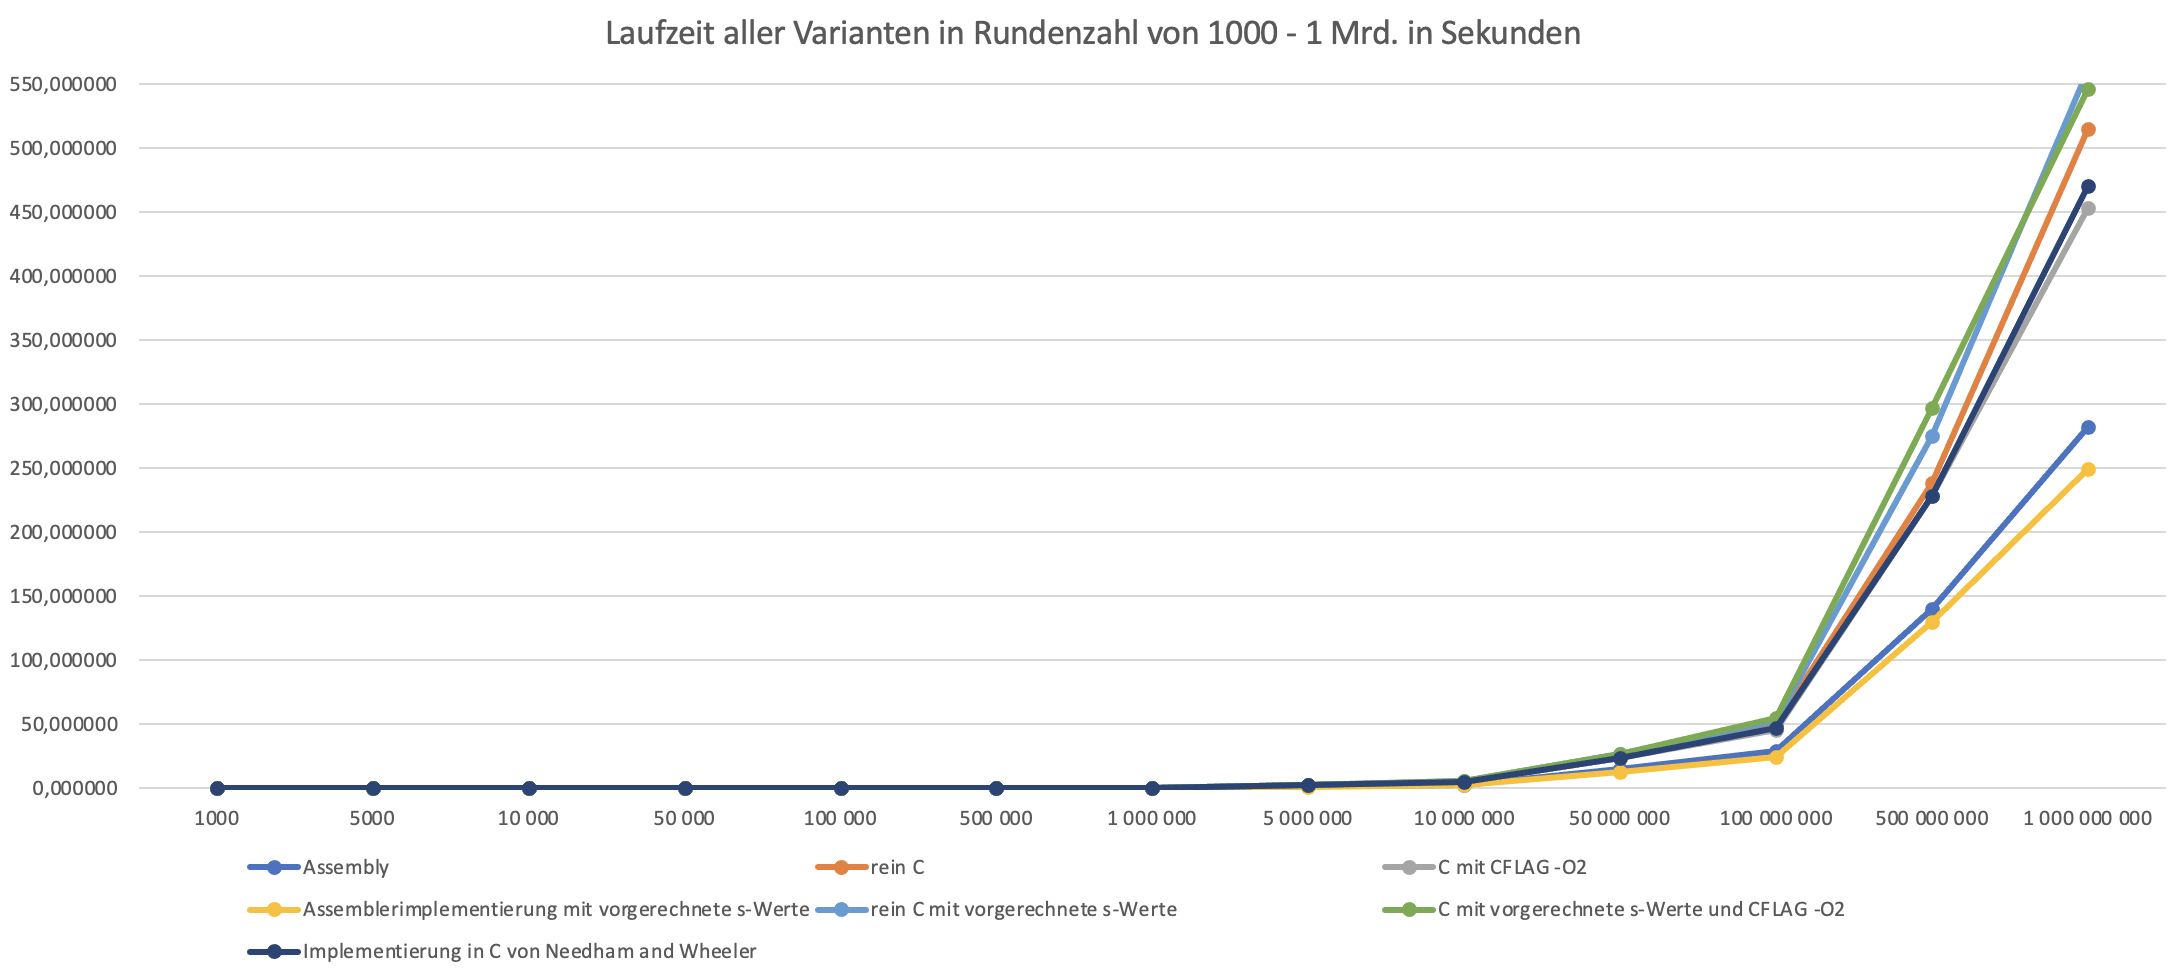
\includegraphics[scale = 0.4]{Analyse.png}
\caption{Laufzeit aller Varianten in Rundenzahl von 1000- 1Mrd in Sekunden als Graph}
\end{figure}
\newpage

Der Grund der fast verdoppelten Laufzeiten aller C-Implementierungen sind die mehrmaligen Speicherzugriffe des compilierten Codes und das Nutzen des 64-bit long integers für die Variable s.

\section{Zusammenfassung und Ausblick}
XTEA ist ein Ver -und Entschlüsselungsalgorithmus der auf der Struktur der Feistelchiffre basiert und eine weitere Entwicklung von TEA ist. Er ist besonders geeignet für größere Datenblöcke. ~\cite{appel2016sicherheitsaspekte}
XTEA ist einfach zu implementieren außer der Zuweisungen besteht XTEA nur aus einem einzigen For-Loop und drei Operationen. Dennoch ist die Verschlüsselung sehr komplex. Es ist auch möglich XTEA in alle Programmiersprachen zu implementieren.
Zur Verbesserung des Algorithmus wurde das Padding mit dem PKCS\#7 Verfahren sowie das logische Shiften von Blöcken verwendet.
Was die Performanceanalyse zeigt stimmt mit unseren Erwartungen überein. Die Erweiterung von der vorgerechneten Variable s hat einen Einfluss auf die Laufzeit. Denn wenn der Algorithmus mit einer vorgerechneten Variable s durchführt wird, nimmt die Lauftzeit ab, wie von uns erwartet. Ebenfalls kann man auch sagen, dass der Algorithmus eine hohe Performance besitzt da dass auch ein Ziel von TEA ist. ~\cite{appel2016sicherheitsaspekte}

\newpage
\section{Bildquellen}
Abbildung 1: https://www.hsg-kl.de/faecher/inf/krypto/feistel/index.php (23.01.2022, 18:23) \\
Abbildung 2: https://www.researchgate.net/figure/Fig-1Two-Feistel-rounds-one-cycle-of-XTEA-III-EXISTING-ATTACKS-ON-XTEA-There-exist\_fig2\_229480139 (27.01.2022, 12:17)\\
% TODO: Fuegen Sie Ihre Quellen der Datei Ausarbeitung.bib hinzu
% Referenzieren Sie diese dann mit \cite{}.
% Beispiel: CR2 ist ein Register der x86-Architektur~\cite{intel2017man}.

%%TODO
\bibliographystyle{plain}
\bibliography{Ausarbeitung}{}

\end{document}
